\subsection{Product perspective}
Domande utili per UML:
\begin{enumerate}
      \item C'è una relazione 1:1 tra CPO e CPMS oppure un CPO è una compagnia che gestisce tante stazioni di ricarica?
            \\ Per ogni CPO c'è un CPMS che amministra PIÙ stazioni di ricarica
      \item Mi immagino il CPMS come una periferica che ha ogni stazione a disposizione, l'UML mostra la struttura dati / funzionale del sistema eMSP, quindi non ha la facoltà di aggiornare attivamente i componenti come CPMS e socket. Vogliamo includere un'interfaccia che permetta a questi componenti di fare una richiesta al server per aggiornare i dati?\\
            Per quanto riguarda l'utilizzare un'altra interfaccia pensavo di inserire un'interfaccia che permettesse di interfacciarsi con il CPMS e con i vari sockets del modello centralizzato. In questo modo non si intaccherebbe l'interfaccia utente e ci sarebbe modo di avere un "filo" di ragionamento coerente con il modello e con la rappresentazione fisica.
      \item Il pattern più comodo per il sistema sarebbe partire sempre da una richiesta del client e poi rispondere. Mi chiedo quindi se è possibile seguire questo profilo in tutto il progetto. Per il calendario pensavo che il client (leggermente fat) potesse chiedere ogni tot al server se sarebbe un buon momento per fare rifornimento ed il server risponde.
\end{enumerate}
\begin{figure}[h!]
      \begin{center}
            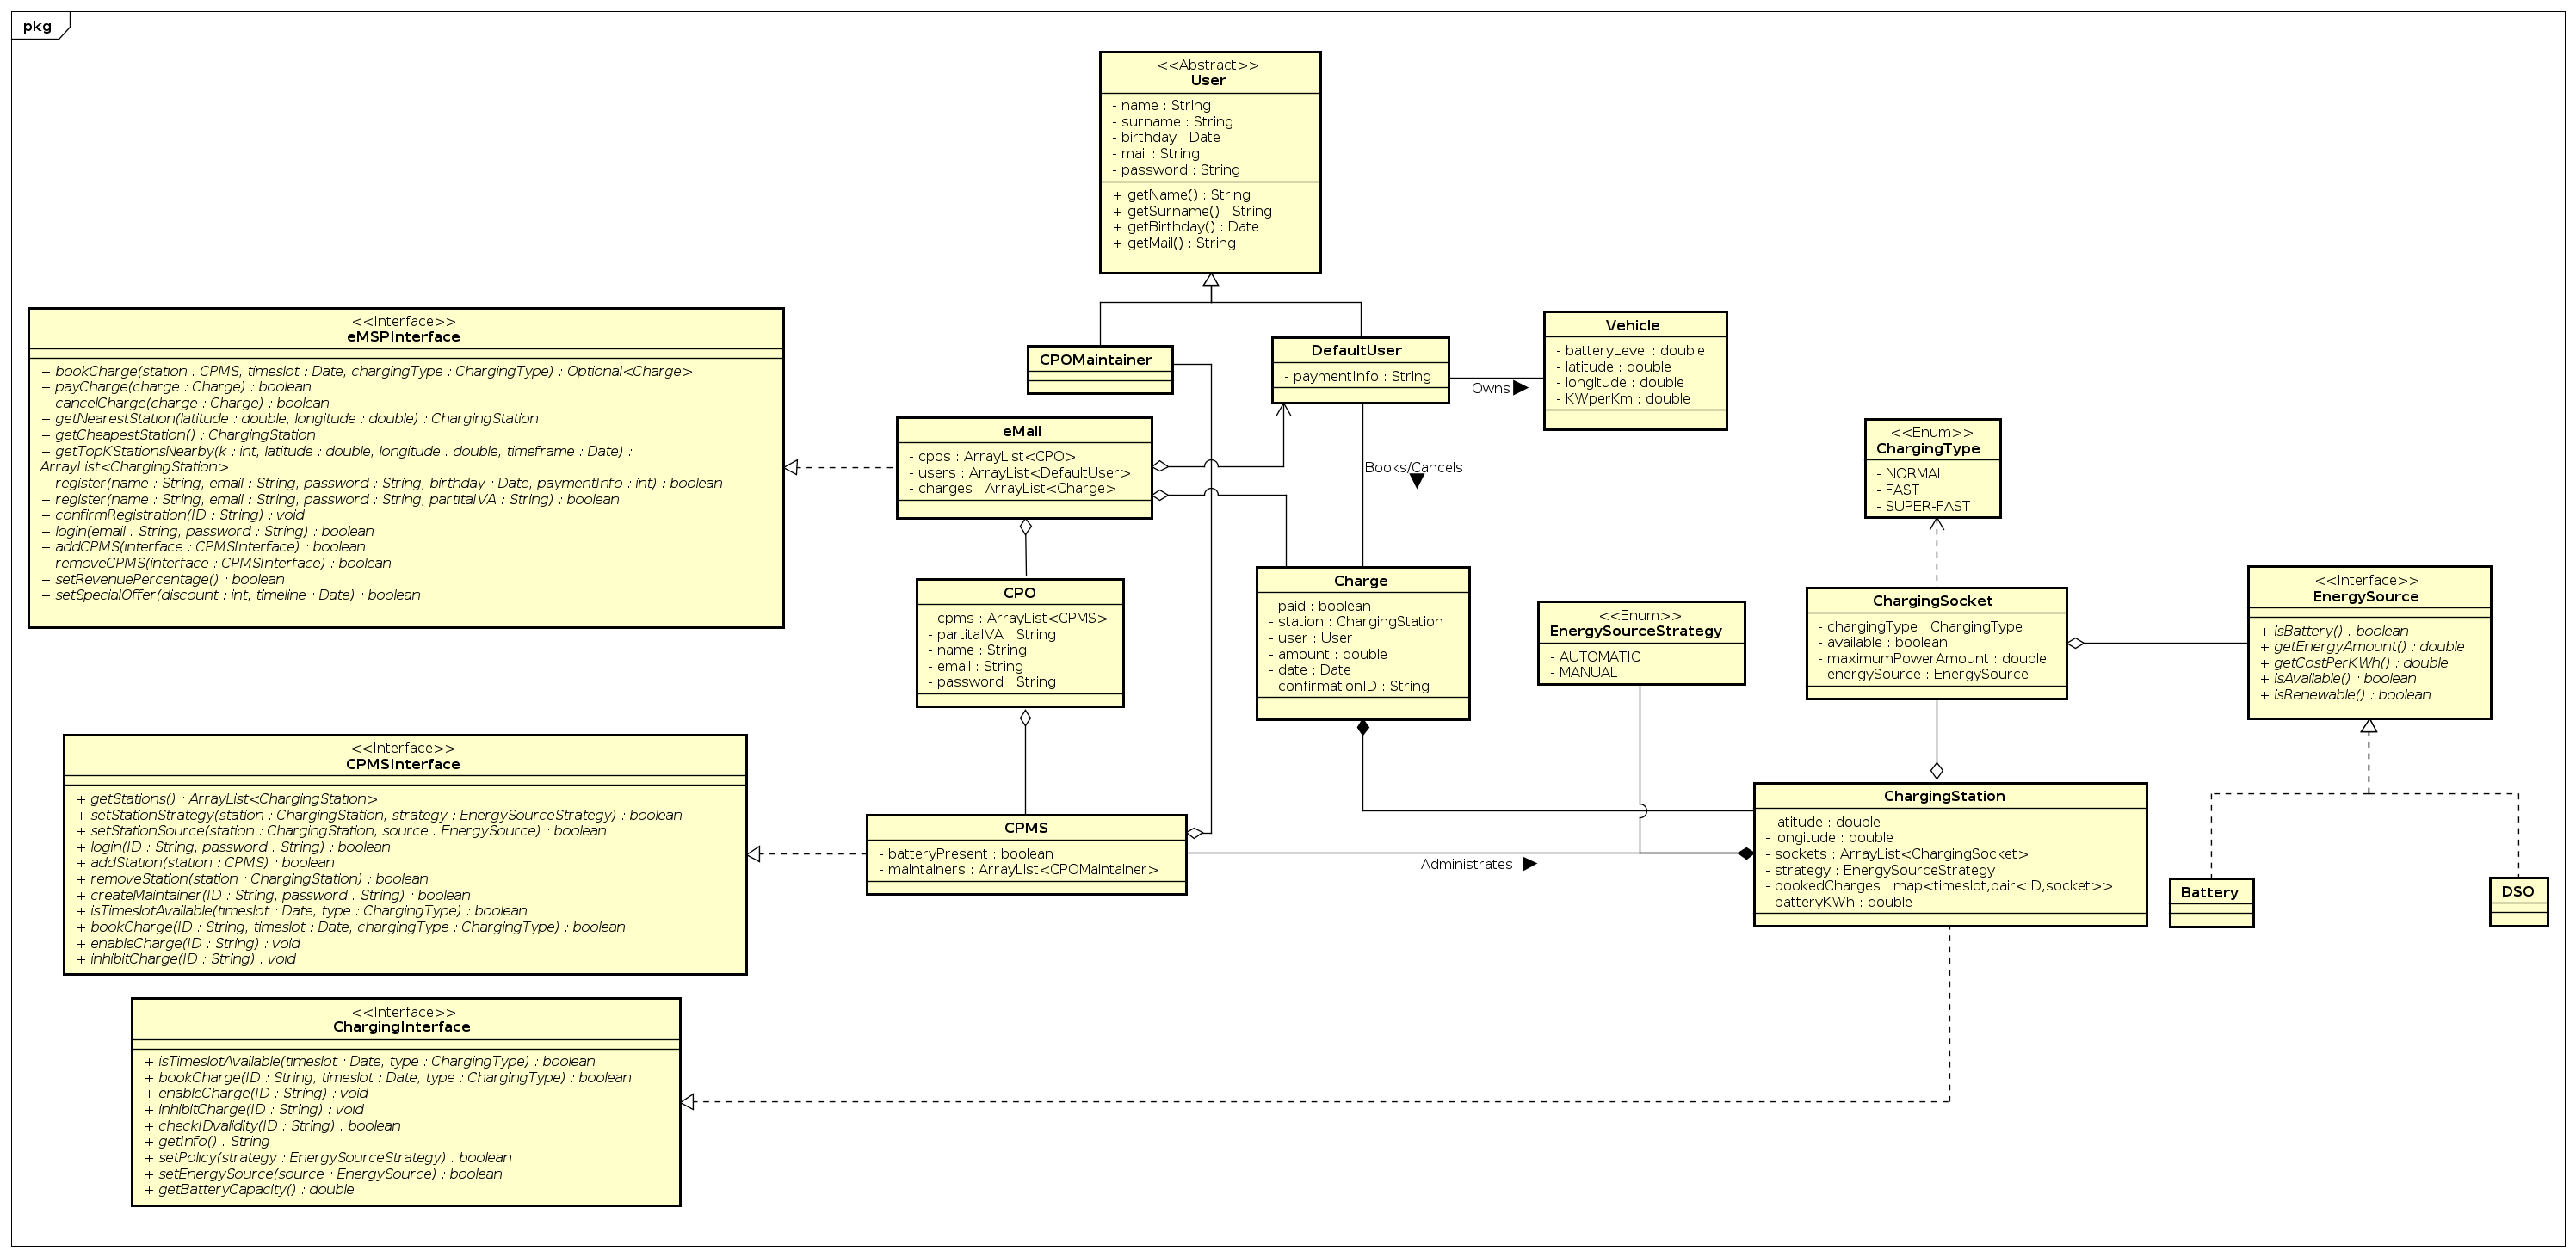
\includegraphics[keepaspectratio, width=16cm]{UML.png}
            \caption{UML}
      \end{center}
\end{figure}
\subsection{Product functions}

\subsubsection{Scenarios}
\begin{enumerate}[label=S\arabic*]
      \item User Signs up:\\
            Lucy, wanting to use the system, opens the app, she is prompted to login or register,
            she chooses to register herself and inserts her personal info (email, password, payment information);
            an email is sent with a link to confirm the activation of the account, if the link is clicked within
            the first 15 minutes the account is activated and the sign up is successful,
            otherwise it is considered failed and the process must be repeated.
      \item User Logs in:\\
            Jay, after signing up, opens the app and he is prompted to insert his email and password,
            if the given information are correct the login is successful and he obtain access to his account
            and the service of the apps, otherwise the login is unsuccessful and it must be repeated.
      \item User searches for stations:\\
            Robert, once logged in, inserts the location and the time frame to search for charging stations.
            Once submitted a list of available charging station is displayed, the list is ordered by the distance of the station
            from the desired location. Via a menu Robert can choose to order the station either via distance or price,
            or to display unavailable station and set the maximum distance from the chosen location.
            Robert chooses a station obtaining more detailed information.
      \item User books a charge:\\
            Jessica, after choosing a station, decides to book it, the station location and booked time frame are displayed
            and she is asked to confirm the booking via a popup. Jessica then receives a confirmation email with the details
            of the charge (Location, time frame, socket id) and a confirmation pin to insert at the station.
      \item User charges the car:\\
            Mary, after booking a charge, arrives at the station, she parks her car at the designed socket
            and plugs her car in, Mary then inserts the confirmation pin in the socket to start the charge.
            The socket displays on a monitor the status and the finishing time of the charge.
            Once the charge is finished Mary receives a notification of finished charge,
            she gets her car and complete the charge.
      \item User gets charging suggestion based on his calendar:\\
            Josh is a very busy man, is also an avid google calendar user,
            setting up every event with correct time and locations.
            The service accessing his calendar finds the closest available charging station to each car movement,
            it estimates the battery level trough the gps data and once the battery is below fifty percent Josh gets notified
            about the possibility to charge his car.
            Josh liking the idea open the app and confirms the booking.
      \item Cpo subscribes to the system:\\
      \item Cpo updates info about its charging stations:\\
      \item Cpo decides the policy to be applied:\\
      \item Cpo checks internal info about the selected charging station:\\
\end{enumerate}
\subsection{User characteristics}

\subsection{Assumptions dependencies and constraints}
\subsubsection{Assumptions}
\begin{enumerate}[label=A\arabic*]
      \item Users insert correct data in the forms
      \item Le persone non trollano
\end{enumerate}
\clearpage